\section{Tenses in French}

There are eight tenses in French:

\begin{itemize}
\item{Pr\'esent - Present}
\item{Imparfait - Imperfect}
\item{Pass\'e simple - Preterite, Simple past}
\item{Pass\'e compos\'e - Present perfect}
\item{Plus-que-parfait - Past perfect}
\item{Pass\'e ant\'erieur - Past anterior}
\item{Futur - Future}
\item{Futur ant\'erieur - Future perfect}
\end{itemize}


\subsection{The Present (Le Pr\'esent)}

The French present tense is similar in usage to the English present tense.
In French, the present tense is used to express all of the following:

\begin{enumerate}

\item{\textbf{Current actions and situations:}\\
Je suis fatigu\'{e}.\\
I am tired.\\\\
Nous allons au march\'{e}.\\
We are going to the market.}

\item{\textbf{Habitual actions:}\\
Il va \`{a} l'\'{e}cole tous les jours.\\
He goes to school every day.\\\\
Je visite des mus\'{e}es le samedi.\\
I visit museums on Saturdays.}

\item{\textbf{Absolute and general truths:}\\
La terre est ronde.\\
The earth is round.\\\\
L'\'{e}ducation est importante.\\
Education is important.}

\item{\textbf{Actions which will occur immediately:}\\
J'arrive !\\
I'll be right there!\\\\
Il part tout de suite.\\
He is leaving right away.}

\item{\textbf{Conditions, such as in si clauses:}\\
Si je peux, j'irai avec toi.\\
If I can, I will go with you.\\\\
Si vous voulez.\\
If you like.}
\end{enumerate}

\noindent The formation is as follows:\\

\textbf{\emph{Subject + Verb Conjugation + Object}}.

\vspace{0.2in}
\noindent \textbf{Negation}\\\\
\textbf{\emph{Subject + ne + Verb Conjugation + pas + Object}}.

\subsection{The Near Future (Le Futur Proche)}

It is used for events which are going to happen in near future.
The formation is as follows:\\

\textbf{\emph{Subject + Aller + Infinitive Verb}}.

\vspace{0.2in}

\noindent \textbf{Negation}\\\\
\textbf{\emph{Subject + ne + Aller + pas + Infinitive Verb}}.

\noindent \textbf{Examples:}\\\\
Je vais voir Luc.\\
I'm going to see Luc.\\\\
Il va arriver.\\
He's going to arrive.\\\\
Nous allons manger.\\
We're going to eat.

\subsection{The Past Compound (Le Pass\'e Compos\'e)}
\label{sec:pastTense}
It is used for events which are complete and that are done in the past.
The formation is as follows:\\

\textbf{\emph{Subject + avoir/\^etre + Past Participle of Verb}}.\\

\noindent The verb \emph{\^Etre} is used with only the following sixteen verbs:\\\\

\begin{tabular}{| r | l | l | l |}
\hline
S.N.  & Verb            & Meaning             & Part Participle \\
\hline
1     & \ul{D}escendre  & To go down, descend & Descendu        \\
2     & \ul{R}entrer    & To return (home)    & Rentr\'e        \\
3     & \ul{M}onter     & To climb, go up     & Mont\'e         \\
4     & \ul{R}etourner  & To return           & Retourn\'e      \\
5     & \ul{S}ortir     & To go out           & Sorti           \\
6     & \ul{V}enir      & To come             & Venu            \\
7     & \ul{A}ller      & To go               & All\'e          \\
8     & \ul{N}a\^itre   & To be born          & N\'e            \\
9     & \ul{D}evenir    & To become           & Devenu          \\
10    & \ul{E}ntrer     & To enter            & Entr\'e         \\
11    & \ul{R}ester     & To stay, remain     & Rest\'e         \\
12    & \ul{T}omber     & To fall             & Tomb\'e         \\
13    & \ul{R}evenir    & To come back        & Revenu          \\
14    & \ul{A}rriver    & To arrive           & Arriv\'e        \\
15    & \ul{M}ourir     & To die              & Mort            \\
16    & \ul{P}artir     & To leave            & Parti           \\
\hline
\end{tabular}

\vspace{0.2in}

\noindent Apart from verbs \emph{Devenir} and \emph{Revenir}, the above 14 verbs
can be easily remembered with help of Figure (\ref{fig:pastTenseEtreVerbs}).

\begin{figure}[!h]
\centering

\includegraphics[height=0.4\textheight]{images/DrMrsVandertramp.jpg}
\caption{DRMRSVANDERTRAMP}
\label{fig:DRMRSVANDERTRAMP}

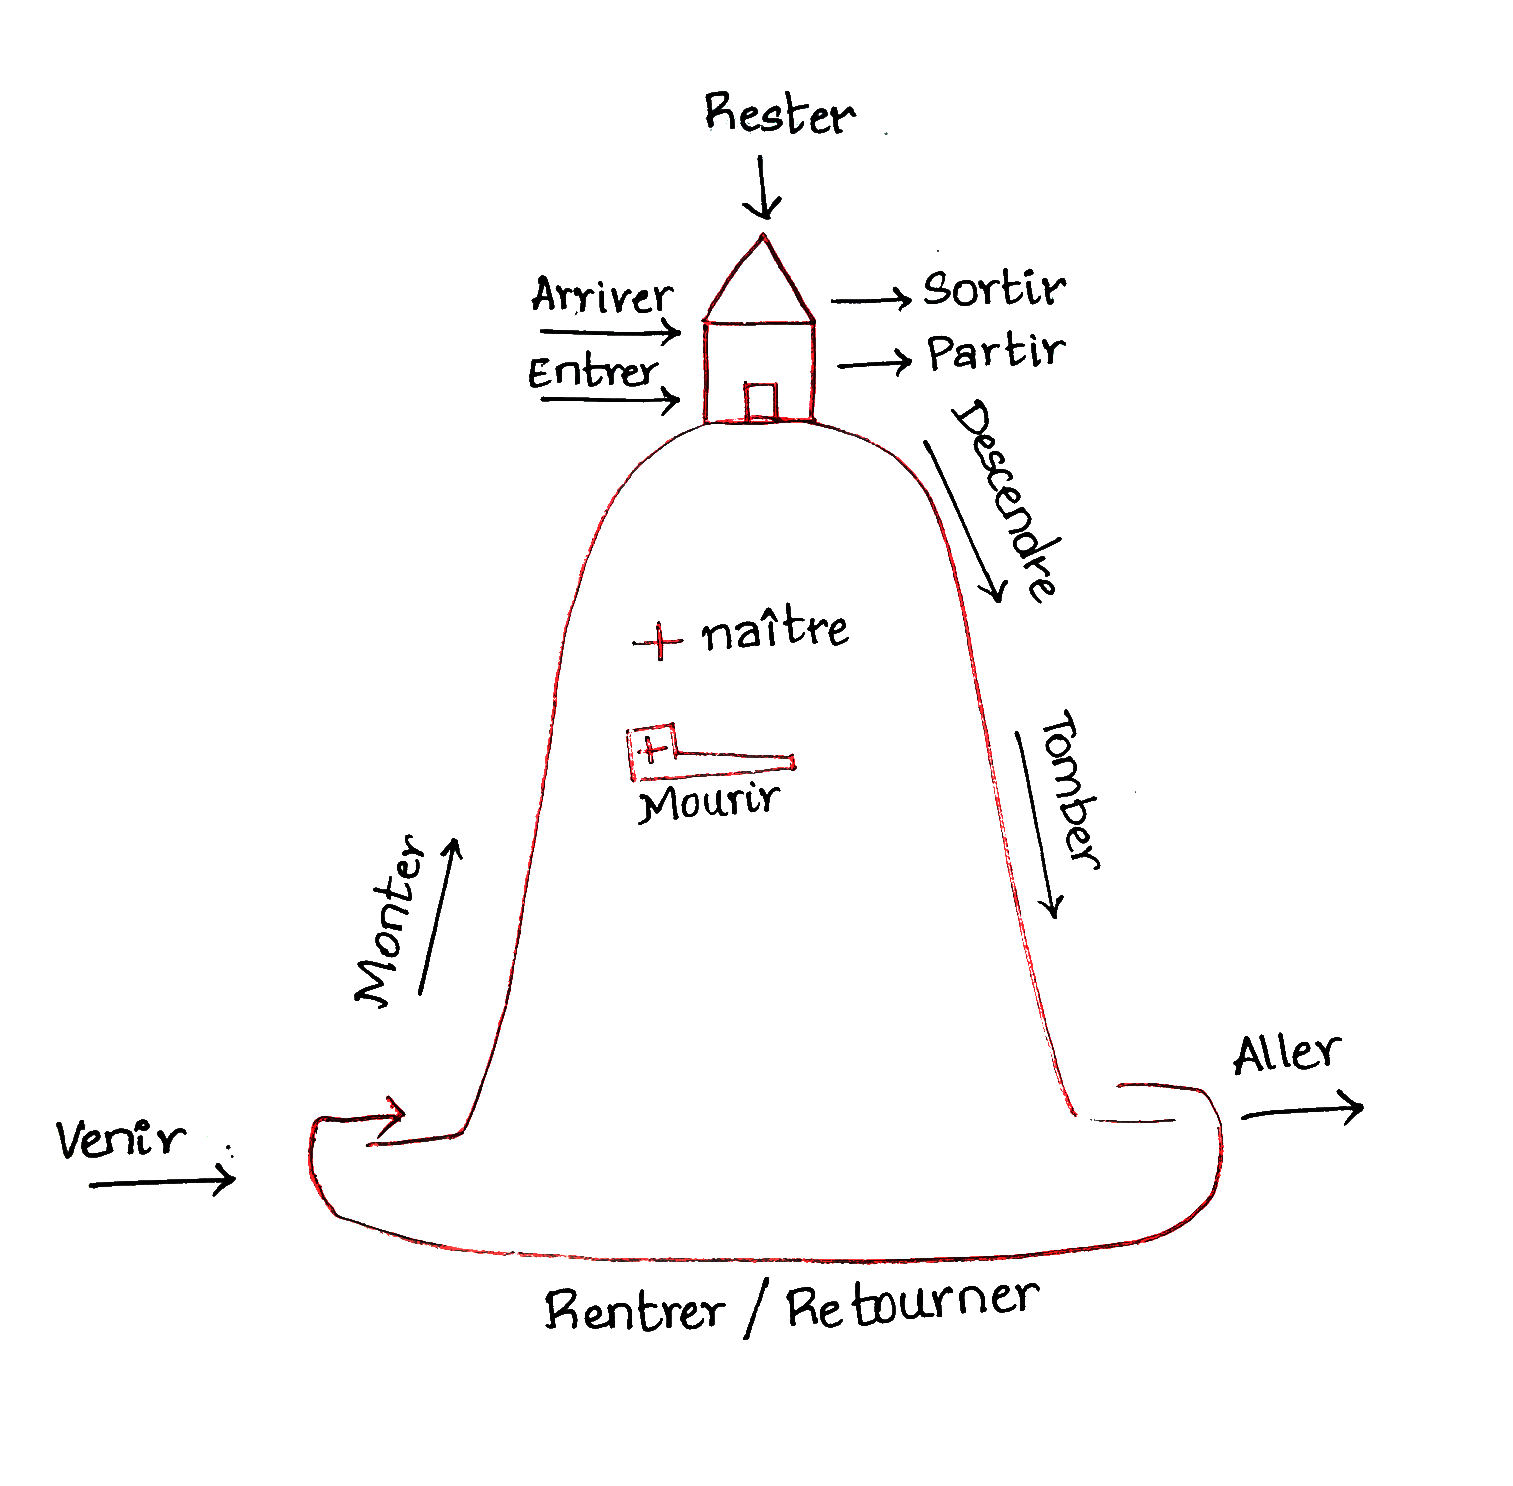
\includegraphics[width=0.4\textheight]{images/PastTense.png}
\caption{Easy way to remember verbs with which \^Etre is used. Notes: Chandana}
\label{fig:pastTenseEtreVerbs}
\end{figure}


\noindent Past participle of the verb \emph{Avoir} is used with all other verbs.
The following table presents many common verbs and their past participle form.\\\\

\begin{longtable}{| l | l | l |}
\hline
Verb            & Meaning             & Part Participle \\
\hline
\endhead
\^etre        & to be       & \'et\'e     \\ \hline
avoir         & to have     & eu          \\ \hline
poser         & to put      & pos\'e      \\ \hline
finir         & to finish   & fini        \\ \hline
faire         & to do       & fait        \\ \hline
jouer         & to play     & jou\'e      \\ \hline
conna\^itre   & to know     & connu       \\ \hline
vouloir       & to want     & voulu       \\ \hline
rencontrer    & to meet     & recontr\'e  \\ \hline
devoir        & to have to  & d\^u        \\ \hline
savoir        & to know     & su          \\ \hline
pouvoir       & can         & pu          \\ \hline
lire          & to read     & lu          \\ \hline
\'ecouter     & to hear     & \'ecout\'e  \\ \hline
r\'epondre    & to answer   & r\'epondu   \\ \hline
parler        & to speak    & parl\'e     \\ \hline
r\'ep\'eter   & to repeat   & r\'epet\'e  \\ \hline
regarder      & to watch    & regard\'e   \\ \hline
travoiller    & to work     & travaill\'e \\ \hline
\'ecrire      & to write    & \'ecrit     \\ \hline
voir          & to see      & vu          \\ \hline
pendre        & to take     & pris        \\ \hline
compredre     & to understand  & compris  \\ \hline
apprendre     & to learn    & appris      \\ \hline
dormir        & to sleep    & dormi       \\ \hline
ouvir         & to open     & ouvert      \\ \hline
d\'ecouvrir   & to discover & d\'ecovert  \\ \hline
f\^eter       & to party    & f\^ete      \\ \hline
traivailler   & to work     & travaill\'e \\ \hline
\end{longtable}

\subsubsection{General rules for past participle of verbs}

\begin{itemize}
\item{\textbf{-ER Verbs:} Remove the R and add accent to E (\'e)\\
Aller : All\'e\\
Parler : Parl\'e}
\item{\textbf{-IR Verbs:} Remove the R\\
Sortir : Sorti\\
Partir : Parti}
\item{For \^Etre verbs only, we agree the past participle form according to
the gender and singulair or pluriel\\
Le soir, des copains sont \ul{venus} chez moi.}
\end{itemize}




